\documentclass{beamer}
\usepackage{listings}  

\usetheme{Padova}


\title{Software Verification}
\subtitle{Bounded Box}
\author{Mattia Bottaro - Mauro Carlin}

\date{May, 2018}


\begin{document}

	\maketitle

	\begin{frame}{Outline}
		\tableofcontents
	\end{frame}


	\section{Project}

	\begin{frame}{Project - Domain}
	We have chosen the \textbf{Bounded Box Domain}, which is a parametric restriction of the interval abstract domain $Int$:\\~\\~\\

		 \scriptsize Given $m, n \in \mathbb{Z} \cup \{-\infty,+\infty\}$, then
	 \normalsize

	  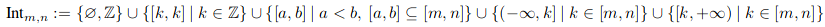
\includegraphics[scale=0.40]{images/consegna.png}
	  	

	\end{frame}
	\begin{frame}{Project - Domain}
		\begin{figure}
			Bounded Box with m = -2, n = 2
			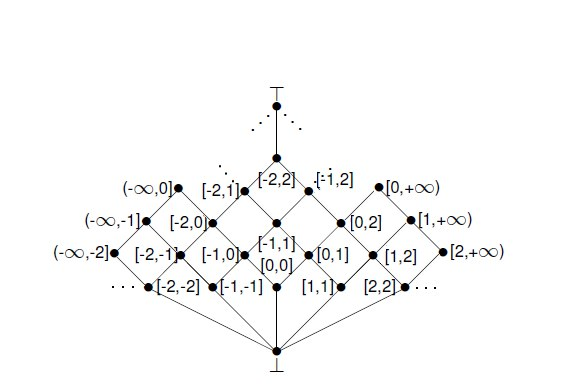
\includegraphics[scale=0.6]{images/box.png}
		\end{figure}

	\end{frame}

	\begin{frame}{Project - Domain}
		\begin{figure}
			Bounded Box with m $>$ n
	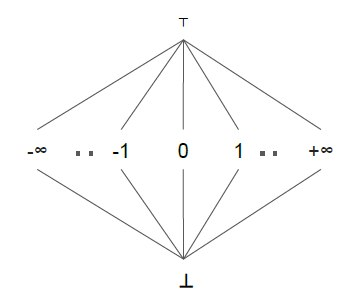
\includegraphics[scale=0.8]{images/constant.jpg}
\end{figure}

\end{frame}

	\begin{frame}{Project - Jandom}
		\begin{itemize}
			\item Static Analyzer for \textbf{Numerical} and Object Domains (forse togliere object)
			\item Jandom was created at the University of Chieti-Pescara
			\item It's a buildup of \textbf{RANDOM}, which analyzes \textbf{R} code
			\item Jandon is written in \textbf{Scala}
			\item Jandom analyzes JVM bytecode using \textbf{Soot}
		\end{itemize}
	\end{frame}

	\begin{frame}{Project - Jandom}
		We've extended Jandom from this repository created by University of Padua' students
		\begin{figure}[c]
			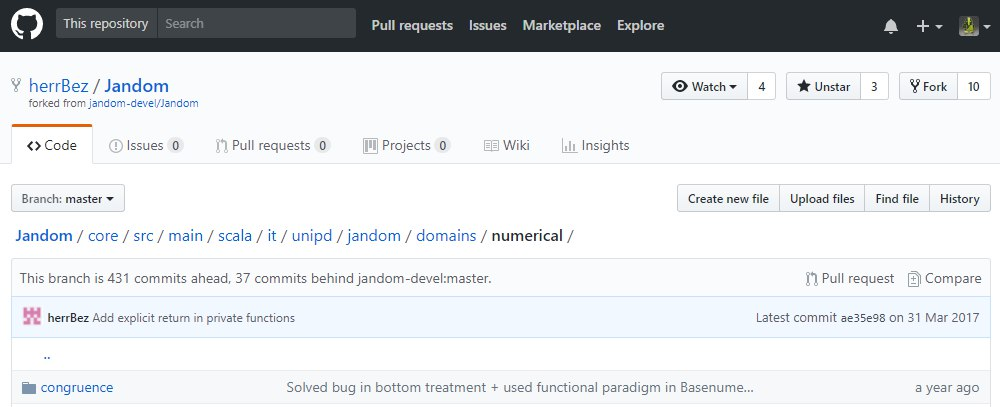
\includegraphics[scale=0.4]{images/repo.jpg}
		\end{figure}
	\end{frame}


	\section{Our Contribution}
	
	\begin{frame}{Our Contribution}

	
	We have:\\
	\begin{enumerate}
		\item Implemented the Integer Interval Domain
		\item Implemented Bounded Box Domain specializing the previous domain, because abstract operators of both domains are very similar
	\end{enumerate}
	
	\end{frame}

	\begin{frame}{Our Contribution}
		Abstract \textbf{sum} operator algorithm in Bounded Box Domain. 
		\begin{enumerate}
			\item Execute sum operator of Interval Domain. \\
			$[a,b] +_{b}^\# [c,d] = [a + c,b + d] = [e,f]$
			\item $[e,f]$ must be represented as an element of Bounded Box Domain
		\end{enumerate}
	\[ [e,f] =
	\begin{cases} 
	\top^\# & e \textless m \land f \textgreater n\\
	[n,+\infty) & e \geq n  \land  e \neq f\\
	[e,+\infty) & e \textless n \land f \textgreater n\\
	(-\infty,m] & f \leq m \land e \neq f\\
	(-\infty,f] & f \textgreater m \land e \textless m \\
	[e,f] & otherwise
	\end{cases}
	\]
		
	\end{frame}
	\begin{frame}{Our Contribution}
		\begin{block}{Abstract \textbf{reminder} operator algorithm in Box Domain}
		\scriptsize	
		\[ [a,b] \%_{b}^\# [c,d] =
		\begin{cases}
		\top^\# & [c,d] = \top^\# \\
		\bot^\# & [a,b] = \bot^\# \lor [c,d] = \bot^\# \lor [c,d] = [0,0] \\ 
		[0,0] & [a,b] = [0,0] \\
		[0,d-1] & c \geq 0\\
		[c+1,0] & d \leq 0 \\
		[c+1,d-1] & otherwise
		\end{cases}
		\]
		\normalsize
	\end{block}
	
	\end{frame}

	\begin{frame}{Our contribution}
		We have defined a new type, called \large\textit{InfInt}\normalsize, to:\\
		\begin{enumerate}
			\item model infinity values with Integer type
			\item overload operations between integer number
			\item simplify further contribution
		\end{enumerate}

	\begin{block}{Example}
		$(+\infty) + n = +\infty$\\
		$(+\infty) \times (-\infty) = -\infty$  \\
		$(+\infty) \div (+\infty) = 0$
	\end{block}
	\end{frame}

	\section{Example}
	
		\begin{frame}{First example}
		
		\begin{flalign}
			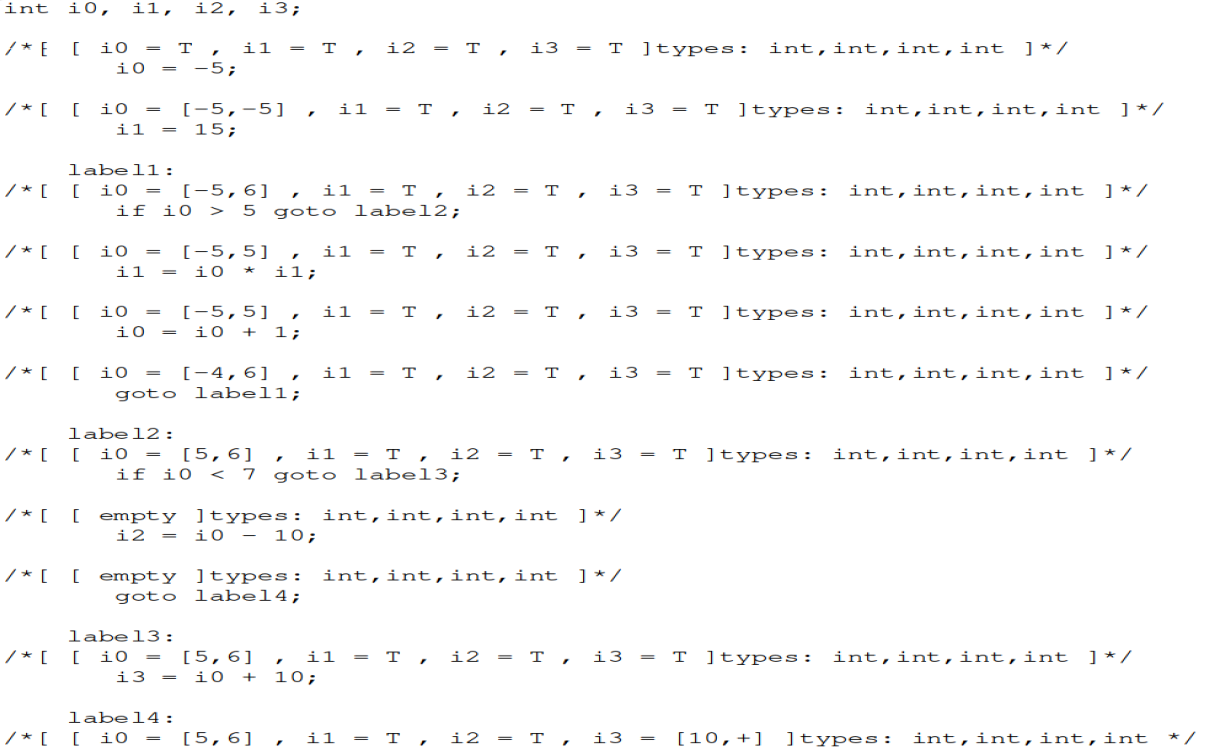
\includegraphics[scale=0.25]{images/firstcode.png}
		\end{flalign}
	
		\end{frame}

	\section{Improvements that could be made}
	\begin{frame}

	\end{frame}

\end{document}
